\section{Preliminary Evidence and Evaluation Plan}
\label{sec:evidence}

\paragraph{On-emulator attack reproduction.} On an Android emulator, an open notification-listener agent read a synthetic OTP from an SMS notification and forwarded it to a loopback endpoint. Across ten independent synthetic canaries, all ten were read and forwarded (observed exposure rate $1.0$ with a Wilson 95\% interval of $[0.72,1.0]$). We then replaced the scripted reader with an off-the-shelf GUI agent (Mobile-Agent v3.5 driven by Claude Sonnet~4.6, screenshot-only observation, no accessibility-tree access) and repeated the same ten-trial protocol: the agent opened the messaging app, read the code off the screen, and typed it into a compose field in all ten trials ($10/10$, Wilson $[0.72,1.0]$), in three to four steps and $42$--$63$~s per trial. Both are functional reproductions of the mechanism, not device results and not paper numbers.

\paragraph{Prototype countermeasure: B0 versus B3.} We built a stock-Android prototype of the mint-and-redact path and measured it against B0 on the same AVD, harness, model, and canary format (Table~\ref{tab:b0b3}). The prototype has three parts: a notification listener that mints an opaque handle (\texttt{SH-XXXXXX}) for a code found in a notification, cancels the original notification, and posts a replacement naming only the source app and the handle; a vault that keeps the plaintext for five minutes and resolves a handle exactly once; and an accessibility service that covers every on-screen node containing a protected value with a non-touchable overlay (Figure~\ref{fig:b3}). With the prototype active the agent read $0/10$ codes (Wilson $[0,0.28]$) and completed $0/10$ tasks; every trial exhausted the six-step budget after long-press, copy-and-paste, contact-avatar taps, and scrolling. A control run with the redaction service disabled by the harness leaked $1/1$ in two steps, so the zero is not a harness artefact. The legitimate path is preserved: the user opens the broker, sees the handle, and taps \emph{Reveal}; the code is shown once, the resolution is audited, and the reveal window is \texttt{FLAG\_SECURE}, hence black in every screen capture. The prototype is not the \texttt{system\_server} design: it covers the notification and screenshot channels, leaves the accessibility tree and the clipboard unmediated, and does not gate reveal on user presence; the result is one emulator image, one model, and ten trials per condition.

\begin{table}[t]
\centering
\small
\caption{Agent-mediated OTP exposure on the same AVD, harness, model, and canary format. Each row is ten trials with a fresh synthetic canary and a six-step budget. B3 is the stock-Android prototype, not the \texttt{system\_server} design.}
\label{tab:b0b3}
\begin{tabular}{@{}lcccc@{}}
\toprule
Condition & Leaks & Exposure & Wilson 95\% CI & Tasks done \\
\midrule
B0 (unprotected) & 10/10 & 1.00 & $[0.72,1.00]$ & 10/10 \\
B3 (prototype)   & 0/10  & 0.00 & $[0.00,0.28]$ & 0/10 \\
\bottomrule
\end{tabular}
\end{table}

\begin{figure}[t]
\centering
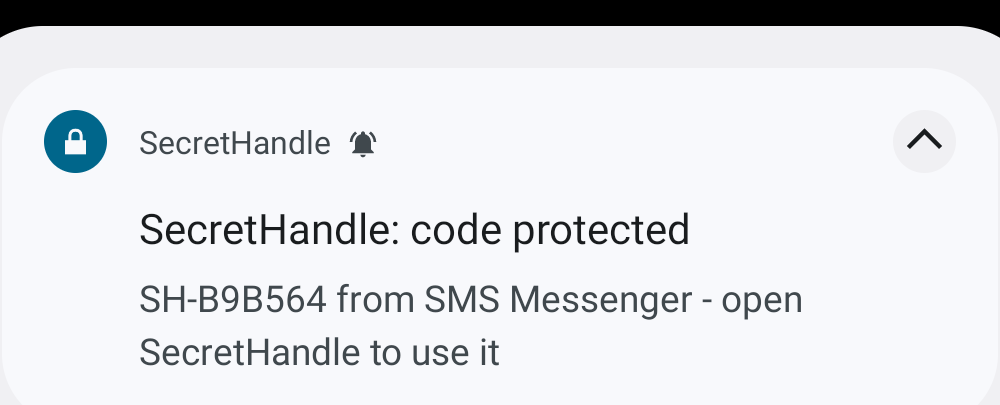
\includegraphics[width=\columnwidth]{../figures/b3_redacted_shade.png}\\[1pt]
{\footnotesize (a) notification shade: source app and handle only}\\[5pt]
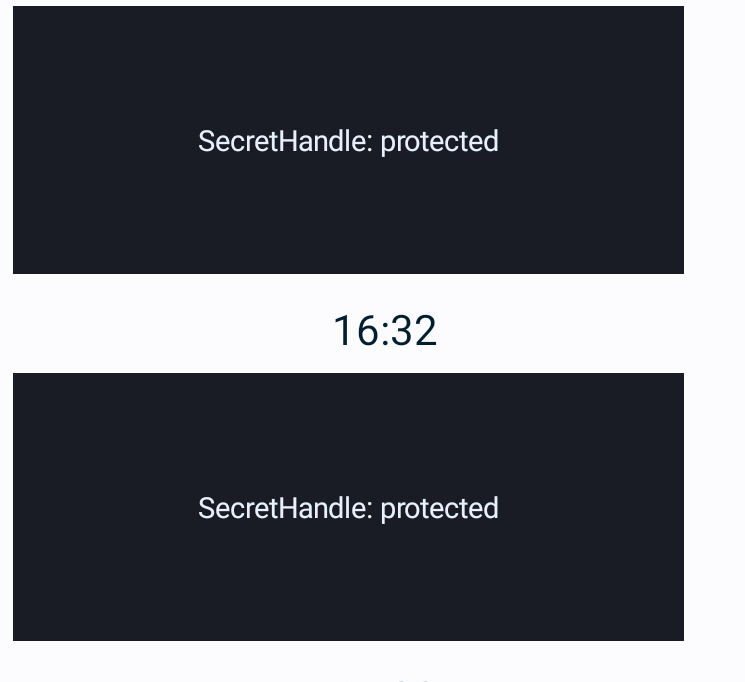
\includegraphics[width=0.55\columnwidth]{../figures/b3_masked_sms.png}\\[1pt]
{\footnotesize (b) conversation view: codes covered by the overlay}
\caption{The B3 prototype on the emulator. (a)~The original notification is cancelled and replaced by one that names the source app and the minted handle; the code is not in the shade. (b)~Each message that carried a code is covered by a non-touchable overlay, so a screenshot-reading agent sees only the marker. The handle is public by design---it is what the user (or an agent) can present to the resolver.}
\label{fig:b3}
\end{figure}

\paragraph{Reference-model study (simulation only).} To check the qualitative trends the design predicts, we ran the project's Python reference model on synthetic canaries (seed \texttt{20261017}, $200$ trials per attack across eight attack families, $6400$ trials total), including read-and-exfiltrate (family~1) and identity ambiguity (family~7). The model is a simulation; its numbers are \emph{not} device measurements and are \emph{not} reported as results. Under it, the unprotected baseline exposed the value in every trial; a detected-placeholder baseline removed the literal value from the immediate artifact but still leaked it after entry (post-entry leakage $1.0$) and still allowed redirection ($1.0$), because it does not bind a destination; and the \SH{} condition produced zero exposure, zero redirection, zero post-entry leakage, zero forgery and replay acceptance, with full legitimate-task success and zero false rejections. On identity ambiguity, \SH{} failed closed (rejected $200/200$) while the baselines delivered the value ($200/200$). The platform-flow baseline was recorded as not applicable because it could not be exercised. Full configuration, outputs, and caveats are in the project's preliminary-evidence document.

\paragraph{Killer experiment (design of record).} The decisive experiment runs the OTP-forwarding injection against an open login-plus-OTP app, first unprotected (the agent forwards the code), then with \SH{}, where the OTP is a handle bound to the login app's package. It passes only if all three hold: (a) the raw code is absent from every instrumented agent artifact; (b) \Enter(handle) into the attacker's destination is rejected by the resolver; and (c) the legitimate login succeeds. In the reference model all three hold; establishing them on a real device is full-paper work.

\paragraph{Research questions.} The full evaluation is organized around six questions: (RQ1) does OS-source minting keep raw values out of all instrumented agent observations and traces? (RQ2) does destination and task binding prevent injection-driven redirection without blocking legitimate completion? (RQ3) do lifecycle and atomic reservation prevent replay, expiry bypass, and concurrency races? (RQ4) does observation redaction prevent post-entry rereading in pixels and accessibility trees? (RQ5) what latency, memory, energy, and interaction overheads arise by source and type? and (RQ6) which identity ambiguities, unsupported apps, WebViews, keyboards, or OEM changes force failure or a weaker policy? RQ1--RQ4 are primary outcomes; the rest are exploratory.

\paragraph{Baselines.} The evaluation compares four conditions: (B0) unprotected, where the agent receives the raw value and types it normally; (B1) a detected placeholder that replaces rendered sensitive text with a local token and resolves it without destination binding, approximating the closest published mobile-placeholder family \cite{zhao2026anonymization}; (B2) the Android platform flow (Autofill, OTP Autofill, or Credential Manager) where the app can invoke it \cite{androidAutofillServices,androidCredentialManager}, with unsupported workflows recorded as not applicable; and (B3) \SH{}. Ablations disable source minting, destination binding, task binding, atomic lifecycle, post-entry redaction, origin checks, or per-use confirmation one at a time, always with synthetic canaries and an isolated endpoint.

\paragraph{Workloads and metrics.} Four open test applications cover username/password plus SMS OTP, multi-page 2FA, address and phone-number checkout, and wallet-token checkout with per-use confirmation; each logs only ground-truth events (target identity, whether a value was delivered, server acceptance, task completion) to a protected harness. For $N$ tasks with instrumented artifact set $I_i$ and canary $s_i$, exposure is $E=\frac1N\sum_i \mathbf 1[s_i\in I_i]$, augmented by normalized, encoded, and substring checks. Redirection $R$ is the fraction of attack trials in which the value reaches a target outside $d$; legitimate utility $U$ is the fraction of benign trials meeting the application oracle; post-entry leakage $L$ counts trials whose value reappears in a later modeled observation; forgery acceptance $F$ and replay acceptance $Y$ count unauthorized injections per attempt. We also record latency (mint, authentication, target lookup, confirmation, injection, redaction), memory, energy where supported, confirmation count, and policy- and false-rejection rates. An observed zero is reported as ``0 of $n$'' with a confidence interval, never as proof that an attack is impossible.

\paragraph{Analysis and sample planning.} General-task regression is measured on AndroidWorld \cite{rawles2024androidworld}, with SPA-Bench \cite{chen2024spabench} for breadth. Binary outcomes receive Wilson confidence intervals; paired comparisons use a paired permutation or exact McNemar test when the assumptions fit; latency uses medians, tail percentiles, and bootstrap intervals. Each condition uses fixed task seeds and paired benign/adversarial versions, blocked by device, agent, model, application, and secret type, with repetitions fixed by a prospective precision analysis before outcomes are seen. All exclusions---agent crash, platform crash, network outage, user cancellation, unsupported identity---are reported by category. Device latency, energy, and hardware-keystore behavior are explicitly deferred and reported only where a suitable device is available.
